\documentclass[a4paper, 12pt]{article}
\usepackage{graphicx}
\usepackage{xspace}
\usepackage[margin= 1in,includefoot]{geometry}
\newcommand\nth{\textsuperscript{th}\xspace}
\usepackage{xcolor}
\usepackage{fancyhdr}
\pagestyle{fancy}
\fancyhead[CE]{Face Mask Detection}
\fancyhead[CO]{Face Mask Detection}
\fancyhead[RE]{}
\fancyhead[RO]{}
\fancyhead[LE]{}
\fancyhead[LO]{}
\fancyfoot[CE]{\thepage}
\fancyfoot[CO]{\thepage}
\fancyfoot[RE]{}
\fancyfoot[RO]{}
\fancyfoot[LE]{}
\fancyfoot[LO]{}
\usepackage{lipsum}
\begin{document}
\begin{figure}

\includegraphics[scale=.43]{medipol.png}
\centering
\end{figure}
\begin{titlepage}
\title{Deep Learning \\ Spring 2021, Project Proposal\\ Face Mask Detection}
\date{Due on Friday April 23\nth, 2021 by 23:59}
\author{by 64160010 - Rumeysa ÇELİK, Istanbul Medipol University}
\maketitle
\end{titlepage}
\tableofcontents
\newpage
\section{\setlength{\parindent}{0pt}{\textbf{INTRODUCTION}}}

As of 2020, the COVID-19 pandemic has been mind-boggling as an event that surprised the world and completely changed it. Strict measures are being taken to prevent the spread of the disease. From the most basic hygiene standards to treatment in hospitals, people are doing their best for the safety of themselves and the community; face masks are one of the personal protective equipment. People wear face masks when they leave their homes, and authorities strictly control people's wearing face masks when in groups and in public places. It is very important to check if people adhere to this basic safety principle. Face mask detector system is applied to control this. Face mask detection means determining whether a person is wearing a mask. The first step in recognizing the presence of a facial mask is detecting the face, which breaks down the strategy into two parts: detecting faces and masks on those faces. \\
In this project, a face mask detector that can distinguish between masked faces and unmasked faces will be developed and the best model will be created for this.
\\
\section{PROBLEM  STATEMENT}

It is mandatory for people to wear face masks when they go out, and authorities should strictly control that people wear face masks in groups and public places. It is very important to check that people are complying with this basic safety principle. To control this, a face mask detector system is applied. The first step in recognizing the presence of a face mask is to identify the face that divides the strategy into two parts: detecting the faces and the masks on those faces. \\In this project, a face mask detector that can distinguish between masked faces and unmasked faces will be developed.
\\Of course, in order to do this, it is very important to have a data set at first.
\begin{figure}[h]
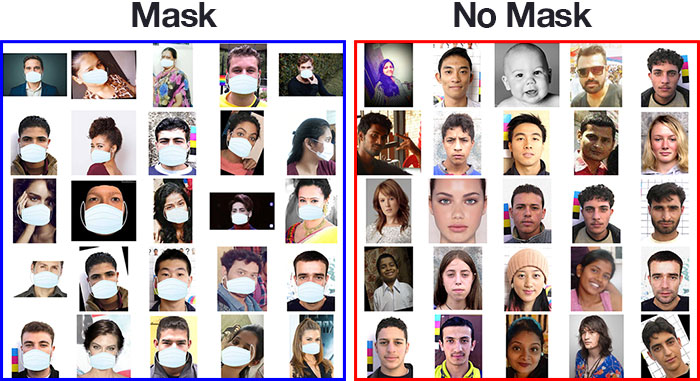
\includegraphics[scale=.43]{1.jpeg}
\centering
\caption{A face mask detection dataset consists of "masked" and "unmasked" images. The dataset will be used to create a COVID-19 face mask detector with computer vision and deep learning using Python, OpenCV, and TensorFlow / Keras.}
\end{figure}
\newpage
The data set to be used for this project is taken from Kaggle.\\ \\
This dataset consists of 3835 images belonging to two classes:
\begin{itemize}
\item with$\_$mask: 1916 images
\item without$\_$mask: 1918 images
\end{itemize}
The goal is to train a specific deep learning model to detect whether a person is wearing a mask or not.
\\
\section{TECHNICAL APPROACH}
\subsection{Convolutional Neural Network Architecture:}
Convolutional Neural Networks are very similar to ordinary Neural Networks in the previous section: they consist of neurons with learnable weights and biases. Each neuron takes some input, performs an inner product, and optionally follows it nonlinearly. The entire network still refers to one differentiable point function: from raw image pixels at one end to class scores at the other end. And in the last (fully connected) layer, they still have a loss function (eg SVM / Softmax) and all the tips / tricks we developed to learn normal Neural Networks still stand.\\ \\
So what is changing? ConvNet architectures make a clear assumption that the inputs are images, which allows us to encode certain properties into the architecture. These then make it more efficient to implement the forward function and greatly reduce the amount of parameters in the network.
\begin{figure}[h]
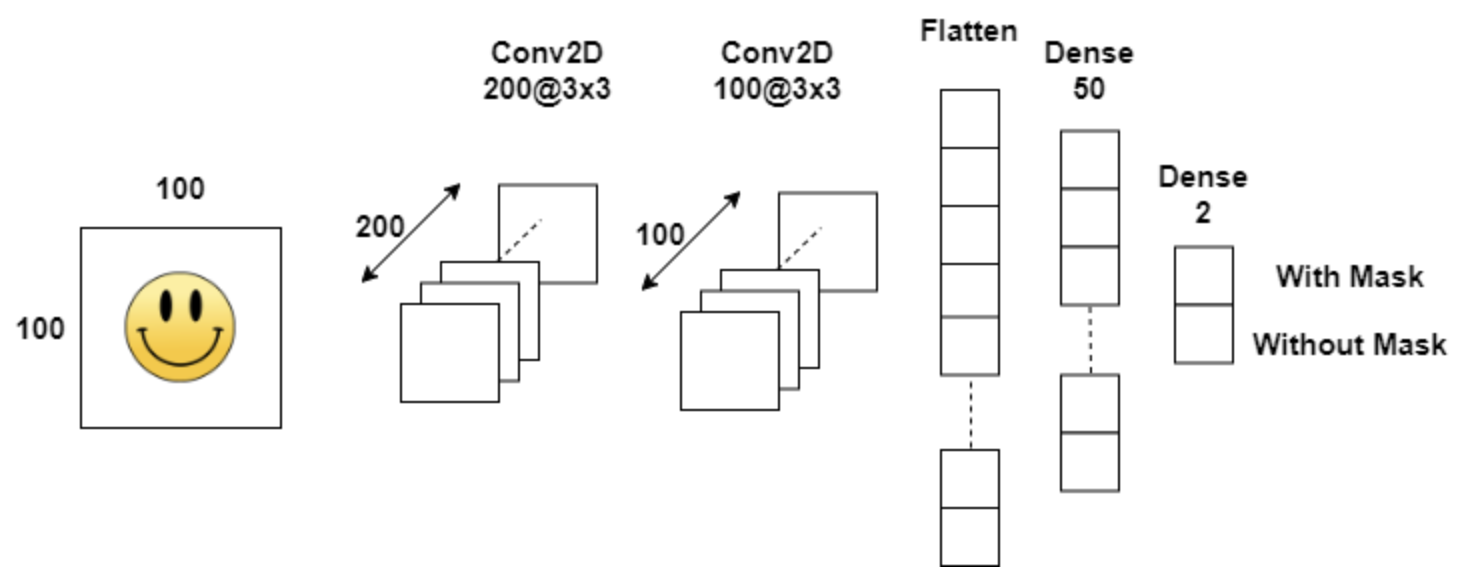
\includegraphics[scale=.43]{2.png}
\centering
\end{figure}
\\
There are parameters that need to be considered while creating a good model.  These are: learning speed, optimization algorithm, epoch number, activation function, dropout value, number of neurons in layers etc.
\begin{itemize}
\item Activation Function:
\\ \\ Activation functions are used to introduce nonlinearity to models, which allows deep learning models to learn nonlinear prediction boundaries.
Generally, the rectifier activation function is the most popular.
Sigmoid is used in the output layer while making binary predictions. Softmax is used in the output layer while making multi-class predictions.
\begin{figure}[h]
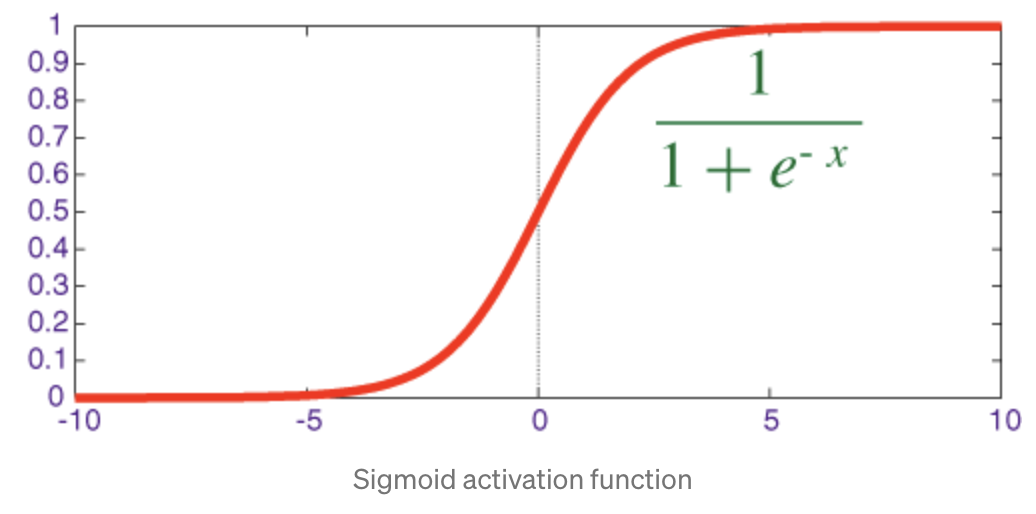
\includegraphics[scale=.43]{3.png}
\centering
\end{figure}
\item Learning Rate:
\begin{figure}[h]
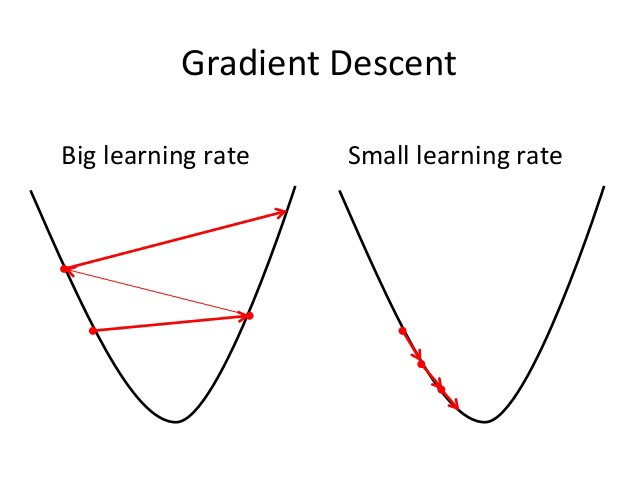
\includegraphics[scale=.43]{4.jpeg}
\centering
\end{figure}
\\
Learning rate defines how quickly a network updates its parameters.
Low learning speed slows down the learning process but merges seamlessly. Higher learning speed accelerates learning but may not converge.
Usually a decaying Learning rate is preferred.\\
\item Momentum:\\ \\
Momentum helps to know the direction of the next step with the knowledge of previous steps. It helps prevent oscillations. A typical momentum selection is between 0.5 and 0.9.\\
\item Number of epochs:\\ \\
The number of epochs is the number of times all training data is shown on the network during training.
Increase the number of epochs until the verification accuracy begins to decrease even when training accuracy increases (overfitting).\\
\item Batch size:\\ \\
Mini batch size is the number of subsamples given to the network after the parameter update has occurred.
A good default for batch size might be 32. Also try 32, 64, 128, 256 and so on.\\
\item Dropout Rate:
\\ \\ The default interpretation of the drop hyperparameter is the possibility to train a particular node in one layer; where 1.0 means no dropout and 0.0 means no exit from the layer.
A good value for a drop in a hidden layer is between 0.5 and 0.8. Input tiers use a larger drop-out rate, such as 0.8.\\
\end{itemize}
Keras is a powerful and easy-to-use free open source Python library for developing and evaluating deep learning models.  \\ In line with the information mentioned above, it is aimed to create the best model.
\begin{enumerate}
\item[1.] Load Data
\item[2.] Define Keras Model
\item[3.] Compile Keras Model
\item[4.] Fit Keras Model
\item[5.] Evaluate Keras Model
\item[6.] Tie It All Together
\item[7.] Make Predictions
\end{enumerate}
\subsection{Detecting Faces with and without Masks:}
\begin{figure}[h]
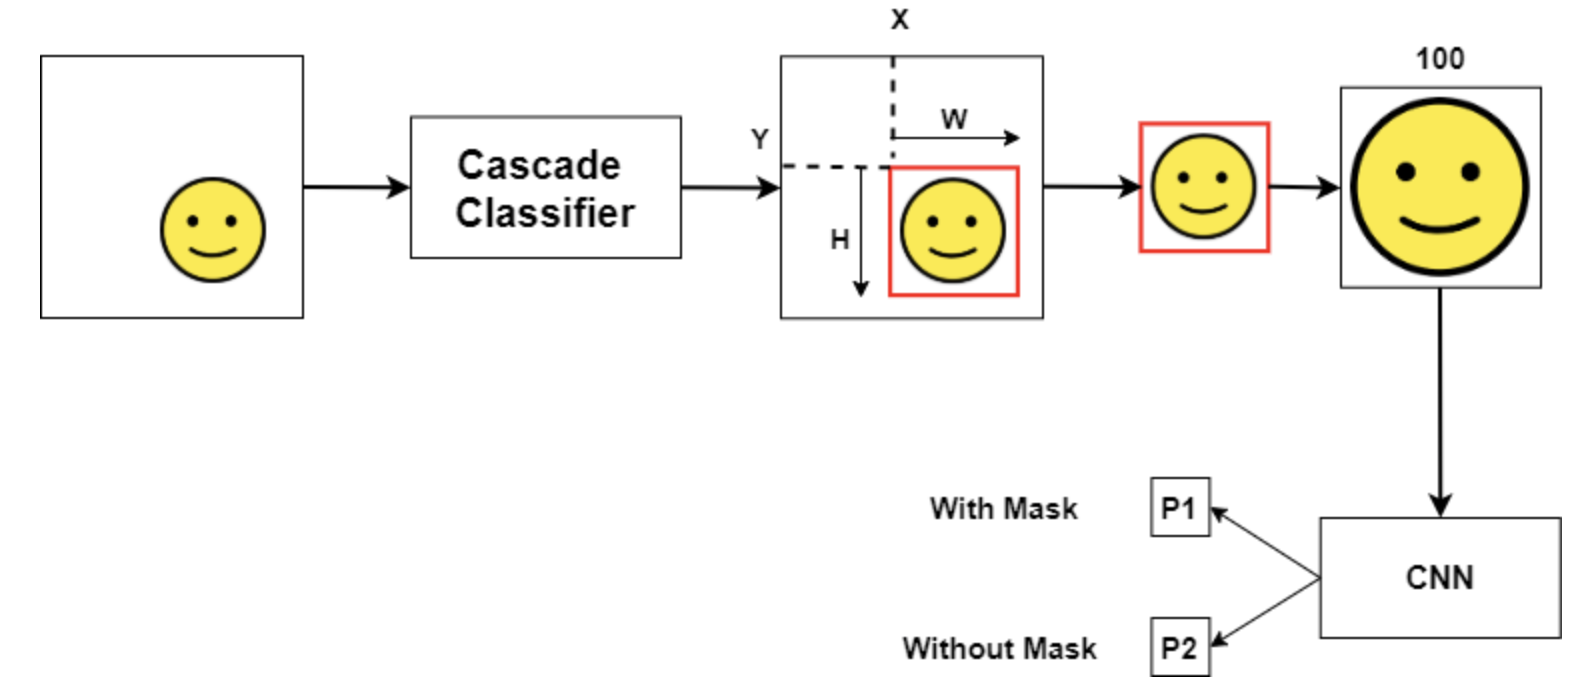
\includegraphics[scale=.41]{5.png}
\centering
\end{figure}
Mask detecting will be performed with opencv by taking the created model. \\ \\
What is OpenCV?\\ \\
OpenCV is a huge open source library for computer vision, machine learning, and image processing, and now plays an important role in real-time operation, which is so important in today's systems. Using it, it can process images and videos to identify objects, faces, and even a person's handwriting. When Python is integrated with various libraries such as Numpy, it can handle OpenCV array structure for analysis. The vector space is used to describe the image pattern and its various properties and mathematical operations are performed on these properties. \\

\section{REFERENCE}
\begin{itemize}
\item https://www.pyimagesearch.com/2020/05/04/covid-19-face-mask-detector-with-opencv-keras-tensorflow-and-deep-learning/
\item https://towardsdatascience.com/what-are-hyperparameters-and-how-to-tune-the-hyperparameters-in-a-deep-neural-network-d0604917584a
\item https://machinelearningmastery.com/tutorial-first-neural-network-python-keras/
\item https://www.geeksforgeeks.org/opencv-overview/
\item https://pythonprogramming.net/convolutional-neural-network-deep-learning-python-tensorflow-keras/
\end{itemize}



























\end{document}